%%%%%%%%%%%%%%%%%%%%%%%%%%%%%%%%%%%%%%%%%%%%%%%%%%%%%%%%%%%%%%%%%%%%%%%%
% UNIBOARD LATEX TEMPLATE
%%%%%%%%%%%%%%%%%%%%%%%%%%%%%%%%%%%%%%%%%%%%%%%%%%%%%%%%%%%%%%%%%%%%%%%%

\documentclass[oneside]{scrreprt}

\usepackage{listings}
\usepackage{import}
\import{latex/}{english.tex} 
% you must set the path according to the current document folder
% use "german.tex" for documents in german and "english.tex" for
% documents in english
\inputpath{{listings/}{figures/}}


% Systems
\newcommand{\univote}{\mbox{UniVote}}
\newcommand{\uniboard}{\mbox{UniBoard}}
\newcommand{\fig}[1]{Figure~\ref{#1}}

\begin{document}

\lstset{
  language=Java,
  basicstyle=\footnotesize\sffamily, %\sffamily, \ttfamily
  keywordstyle=\bfseries,
  numbers=right
}

\title{UniBoard Architecture Specification}
\maketitle

\begin{versionhistory}
	\vhEntry{0.1}{August 13, 2013}{Eric Dubuis}{Initial draft.}
	\vhEntry{0.2}{September 10, 2013}{Eric Dubuis}{Introduced chain of components.}
	\vhEntry{0.3}{February 17, 2014}{Eric Dubuis}{..., removed typos.}
	\vhEntry{0.4}{April 24, 2014}{Severin Hauser}{Made changes so that it corresponds to the formal spec.}
\end{versionhistory}

%%%%%%%%%%%%%%%%%%%%%%%%%%%%%%%%%%%%%%%%%%%%%%%%%%%%%%%%%%%%%%%%%%%%%%%%
%\chapter*{Abstract}
%%%%%%%%%%%%%%%%%%%%%%%%%%%%%%%%%%%%%%%%%%%%%%%%%%%%%%%%%%%%%%%%%%%%%%%%


%%%%%%%%%%%%%%%%%%%%%%%%%%%%%%%%%%%%%%%%%%%%%%%%%%%%%%%%%%%%%%%%%%%%%%%%

\tableofcontents

%%%%%%%%%%%%%%%%%%%%%%%%%%%%%%%%%%%%%%%%%%%%%%%%%%%%%%%%%%%%%%%%%%%%%%%%
\chapter{Introduction}
%%%%%%%%%%%%%%%%%%%%%%%%%%%%%%%%%%%%%%%%%%%%%%%%%%%%%%%%%%%%%%%%%%%%%%%%

This document presents the architectural specification of \uniboard,
a (rather) universal public bulletin board. Specific to this
architecture specification is that it defines the \emph{standalone},
monolithic as well as the \emph{distributed} variant of the
public bulletin board.

To achieve this, the following architectural goals have been in mind:

\begin{itemize}
	\item The same specification for the architecture
		of the \emph{standalone} and the \emph{distributed}
		variant of \uniboard.
	\item Establishment of a \emph{component composition} in
		order to achieve the desired functionality.
	\item Plug-in facility to switch from the standalone variant
		to the distributed one, and vice versa.
\end{itemize}

Note that the supported properties of \uniboard\ depend of the combination of components used.

%%%%%%%%%%%%%%%%%%%%%%%%%%%%%%%%%%%%%%%%%%%%%%%%%%%%%%%%%%%%%%%%%%%%%%%%
\chapter{Component Composition}
%%%%%%%%%%%%%%%%%%%%%%%%%%%%%%%%%%%%%%%%%%%%%%%%%%%%%%%%%%%%%%%%%%%%%%%%

In (Ref.\ to be provided), several properties and the basic operations of a public bulletin
board have been identified. We present in this document the
specification of a software architecture allowing to implement
these properties by \emph{composition} of respective building
blocks, the so-called \emph{components}. For every operation a 
\emph{chain of components} is used as the pattern for the
composition.

\uniboard\ consist of one node (for the standalone variant) or
a set of nodes (for the distributed variant). For the
distributed variant, a specific component is inserted
into the chain of components. That component implements
the respective agreement protocol by communicating with
peer nodes.

Each component implements at least one of the generic service interfaces.
This allows the desired chains of components. (Of
course, not every arbitrary combination of components results
in a useful configuration.) The final component in this chain
is a persistence service allowing to store information, and
to retrieve it later. In fact, our architecture follows the
\emph{chain of responsibility pattern} \cite{Gamma:1995:DPE:186897}.


\section{Chain of Components}

In order to achieve upmost flexibility, the two basic operations of
\uniboard\ are represented with \emph{generic} service
interfaces, simply called \emph{GetService} and \emph{PostService} (namespaces in text
omitted for brevity). That is, each component
implements either one or both interfaces.

The chains of components (Get-Chain and Post-Chain) are achieved by linking a component
to the next one, which in turn is linked to another component.
Only the last component in the chain, the \emph{PersistenceService}, is not
linked anymore to another component. \fig{fig:chain-of-components}
shows the static structure. 

\begin{figure}[ht]
\centerline{
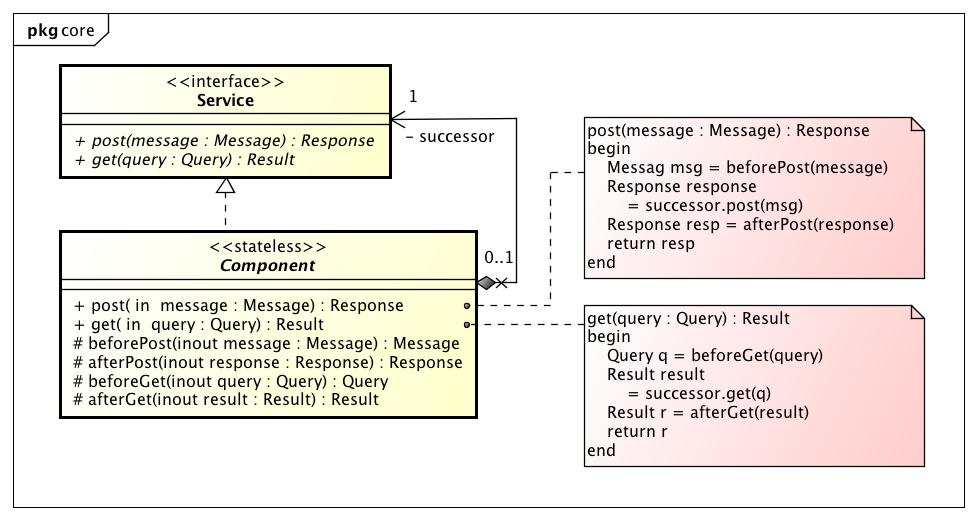
\includegraphics[width=1.0\textwidth]{figs/chain-of-components}}
\caption{UML class diagram defining the interface and linking
of the components. Each component implements the same generic
interface. The Component class, as shown, is abstract. That
implies that concrete components subclass the abstract
Component class.}
\label{fig:chain-of-components}
\end{figure}

The \emph{Service} interface consists of two
general-purpose methods, \emph{post} and \emph{get}:

\begin{lstlisting}[style=javastyle]
package ch.bfh.uniboard;

public interface Service {
    public Attributes post(byte[] message, Attributes alpha, Attributes beta);
    public ResultContainer get(Query query);
}
\end{lstlisting}

Not only the interface is rather generic, but also the provided
and returned data containers \emph{Attributes},
\emph{Query}, and \emph{ResultContainer}. The introduction of generic
data containers minimizes the coupling: Components depend on
the core classes only, but not on specific classes of other
components. See (TODO: Provide Ref.\ to be provided) for
a more detailed elaboration on this topic.

The meaning of the data abstractions can be summarized as follows:

\begin{itemize}
	\item \emph{Attributes:} List of attributes, where each attribute is computed
		by the author or a component. These attributes belong either to a message or result.
	\item \emph{Query:} Data that originates from an author
		for a \emph{get} operation. The \emph{Query} defines the set of posts that are returned as the result.
	\item \emph{ResultContainer:} Consists of two parts. First there is a set of posts that satisfies the \emph{Query}, and there are \emph{Attributes} for this result. Every component may add an attribute. The result is set by the final component, the persistence store.
\end{itemize}


\section{Service Request Delegation}

At start-up time, a board is configured by a number
of concrete components arranged in a chain of component
instances. To service a client, there is at first a \emph{BulletinBoardService}. This service
provides the interface for the client.  It forwards the request to the first
component, which passes it to the next component. It may also process the
service request before passing it to the next
component. Consequently, it may also process the
response before returning it to the \emph{BulletinBoardService}.

\begin{figure}[ht]
\centerline{
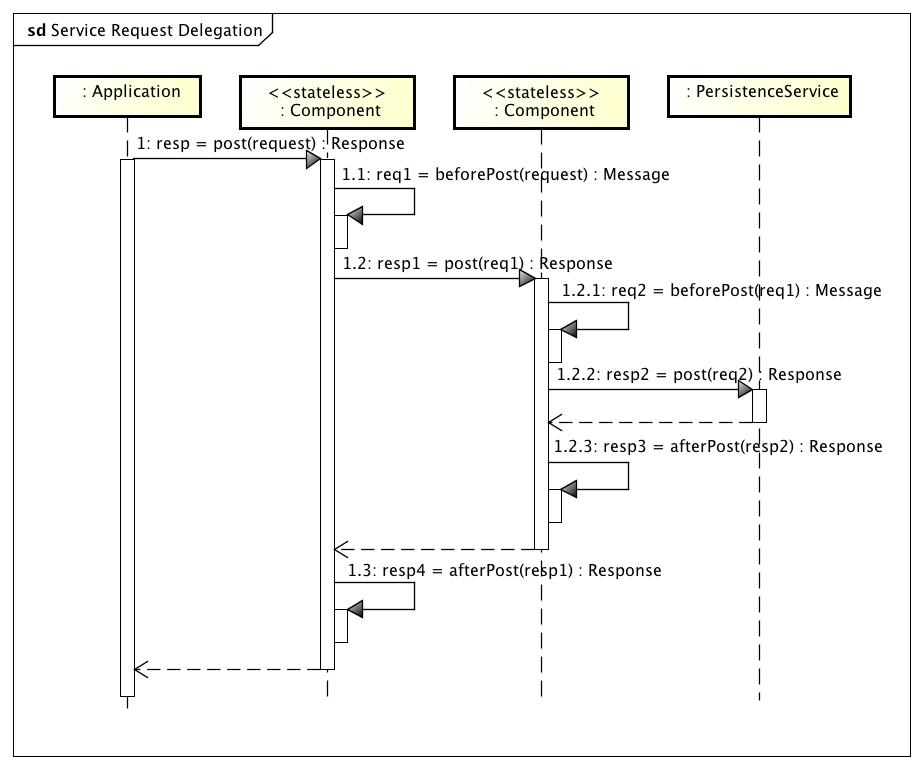
\includegraphics[width=1.0\textwidth]{figs/service-request-delegation}}
\caption{UML sequence diagram illustrating the dynamics of the
delegation of a service request. Each \emph{post()} request received
at a component is processed at first internally by the
self-delegated method \emph{beforePost()}, and then passed to
the next downstream component. The response of the downstream
component is processed at first by the self-delegated
method \emph{afterPost()}, and then returned to the calling
component (or the application).}
\label{fig:service-request-delegation}
\end{figure}

The above described behavioral pattern is repeated with
every intermediate component. Notice that \emph{synchronous} calls
are used between the components.
However, asynchronous processing may occur within
a component, which will likely be the case for the
distributed variant of the board.

\section{Handling Service Requests}

A \emph{BulletinBoardService} or a component requests a service provided by
the downstream component. Basically, the following three
processing actions will occur in the downstream component:

\begin{enumerate}
	\item The received request is processed.
	\item The processed request is passed to the downstream
		component.
	\item The result of the downstream component is
		processed and returned to the calling
		component (or the application).
\end{enumerate}

The comments of \fig{fig:chain-of-components} sketch
the above described processing actions. The template \cite{Gamma:1995:DPE:186897}
of this behavior is predefined in the abstract class Component:

\begin{lstlisting}[style=javastyle]
package ch.bfh.uniboard.service;

public abstract class Component implements Service {
    private Service successor;

	public final Attributes post(byte[] message, Attributes alpha, Attributes beta) {
		Attributes beforePost = this.beforePost(message, alpha, beta);
		...
		Attributes betaReceived = this.getSuccessor().post(message, alpha, beforePost);
		this.afterPost(message, alpha, betaReceived);
		return betaReceived;
	}
    public finalResultContainer get(Query query) {
        // analogous to method post() above
    }
    protected Attributes beforePost(byte[] message, Attributes alpha, Attributes beta) {
        return beta;
    }
    protected void afterPost(byte[] message, Attributes alpha, Attributes beta) {
    }
    // analogous for methods beforeGet() and afterGet()
}
\end{lstlisting}

Subclasses needing to process a message before passing it
to the downstream component merely overwrite method
\emph{beforePost()}:

\begin{lstlisting}[style=javastyle]
package lu.unilu.uniboard.component_x;

import ch.bfh.uniboard.service.*;

public class Component_X extends Component {
    ...
    protected Attributes beforePost(byte[] message, Attributes alpha, Attributes beta) {
        // process given message and attributes
        // (or pass back modified attributes object, not shown)
        return beta;
    }
}
\end{lstlisting}

Similarly, subclasses overwrite methods \emph{afterPost()},
\emph{beforeGet()}, and \emph{afterGet()} in order to implement
the desired behavior.


\section{Generic Data Container}
The generic data containers are not only used to transmit data from component to component, but also for the communication with the users of UniBoard.

\subsection{Attributes}
Attributes is basically 
\subsection{Query}

\subsection{ResultContainer}

%%%%%%%%%%%%%%%%%%%%%%%%%%%%%%%%%%%%%%%%%%%%%%%%%%%%%%%%%%%%%%%%%%%%%%%%
\chapter{Specific Services}
%%%%%%%%%%%%%%%%%%%%%%%%%%%%%%%%%%%%%%%%%%%%%%%%%%%%%%%%%%%%%%%%%%%%%%%%

In order to implement the desired properties of the public bulletin board,
 a number of concrete services are required:

\begin{itemize}
	\item \emph{bfh-webservice} Provides an interface to UniBoard over WebServices.
	\item \emph{Property Service} This service provides properties required by the bulletin board. Its
		realization is composed of a series of property
		implementation, all adhering to the very same
		\emph{Service} interface, exploiting the pluggable
		layered architecture.
	\item \emph{Persistence Service} This service provides
		the view to the persistence storage of the postings
		sent to \uniboard.
\end{itemize}

Some details of the \emph{fault tolerance service} will be described
in the next chapter. Course views for a \emph{property service}
and the \emph{persistence service} are given in the next sections.

TODO: Provide details on accessing the bulletin board.

\section{bfh-webservice}
The module bfh-webservice offers the basic operations introduced in (do Ref) as a webservice.
\begin{itemize}
	\item $\mathrm{Post}(m,\alpha):\beta$
	\item $\mathrm{Get}(Q):R, \gamma$
\end{itemize}

%\section{A Service Implementing a Property}
%
%The public bulletin board requires a number of properties. Our
%architecture implies that each property is realized within
%one component. Since a component requires the service of
%the downstream component, a downstream component is
%linked with the component automatically; the necessary
%code is inherited from the subclass \emph{Component}.
%
%\fig{fig:authorization-service} shows the structure of
%the authorization service.
%
%\begin{figure}[ht]
%\centerline{
%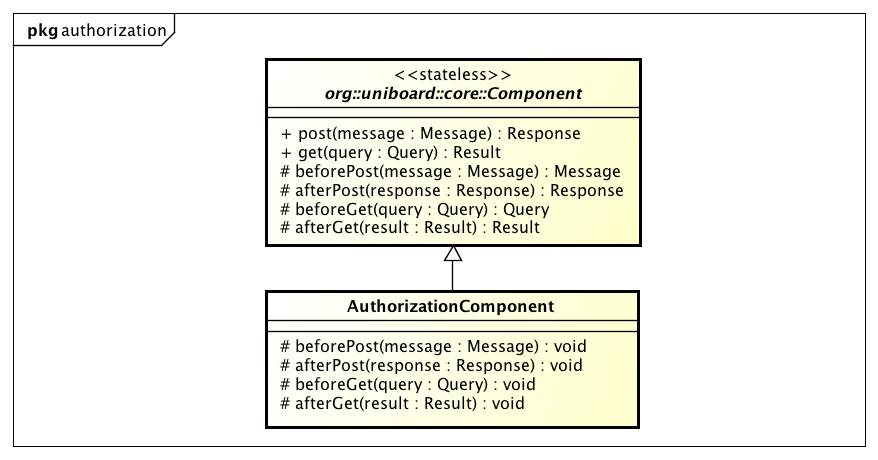
\includegraphics[width=1.0\textwidth]{figs/authorization-service}}
%\caption{UML class diagram for the illustration of the
%authorization service component. Notice that it is derived
%from the \emph{Component} class which implies that there
%is a downstream component link to this component.}
%\label{fig:authorization-service}
%\end{figure}
%
%
\section{The Persistence Service}

The persistence service provides operations to store and
retrieve data. It is a component in the sense that it
implements the \emph{Service} interface. However, it
does not have any downstream component and, thus, cannot be
derived from the \emph{Component} abstraction.

\fig{fig:persistence-service} shows the structure of the persistence service
component.

\begin{figure}[ht]
\centerline{
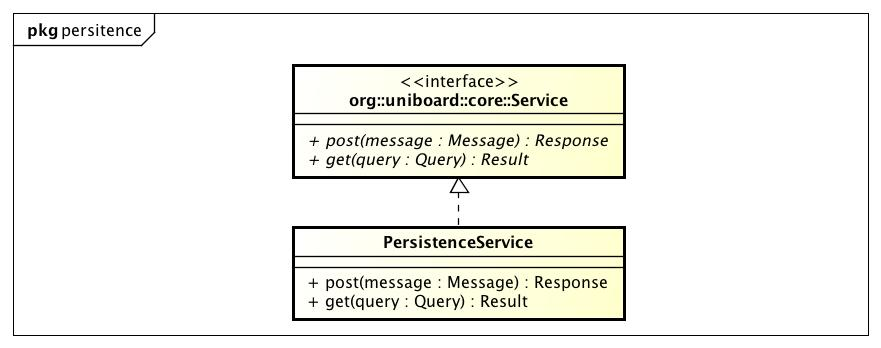
\includegraphics[width=1.0\textwidth]{figs/persistence-service}}
\caption{UML class diagram for the illustration of the
persistence service component. Notice that it merely implements
the \emph{GetService}, \emph{PostService} and \emph{InternalGet} interfaces, and that it is not derived
from the \emph{Component} class.}
\label{fig:persistence-service}
\end{figure}

Data posted and retrieved is called \emph{post}. A post is always constituted of three elements: the \emph{message}, the \emph{alpha attributes} that are post attributes defined by the poster and \emph{beta attributes}, which are attributes defined by the board. The persistence service has to store these three elements.

\subsection{Storing the message}

Our implementation of the persistence service uses MongoDB as database. MongoDB is a JSON document based database. This means that a post must be transformed in a JSON document previous to saving it. This allows to store a JSON structured \emph{message} in a post without having the board knowing the structure of the message in advance. A message must be given in the form of a byte array, this allowing the poster to store everything in the message. If the poster wants to store a JSON structure as message of the post, the poster has to convert the JSON string to a byte array using UTF-8 encoding, before passing it to the persistence service. When the persistence service receives a post to store, it tries to interpret the message as a JSON string. If it successes, it stores the message in that format, otherwise, it stores it as byte array. \\
MongoDB then allows to retrieve a post giving a JSON key and the value it should have. So, a user can retrieve a post by indicating a key used in the message of a post. Therefore, the user must know the structure of the JSON message, but the board doesn't.

\subsection{Storing the attributes}

The attributes \emph{alpha} and \emph{beta} are of type \emph{Attributes} which is a simple class containing a map storing the attributes as key-value pair. Using MondoDB for storing these attributes offers another advantage: the database can accept an undefined number of attributes since they are also stored as JSON elements.

The key of an attribute must be a string. The value however can have different type. An interface called \emph{Value} defines the abstract type of the value, its concrete implementations define the concrete types allowed for an attributes. They are: \emph{StringValue}, \emph{IntegerValue}, \emph{DoubleValue}, \emph{DateValue}, \emph{ByteArrayValue} as shown in \fig{fig:value-type}. All these types are natively supported by MongoDB for storing and querying.

\begin{figure}[ht]
\centerline{
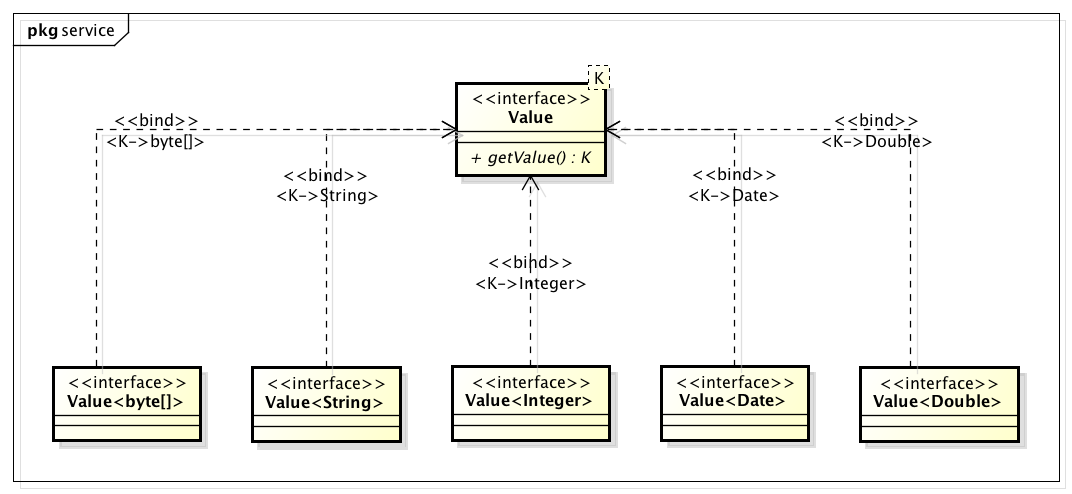
\includegraphics[width=1.0\textwidth]{figs/value_type}}
\caption{UML class diagram variable types allowed for attributes.}
\label{fig:value-type}
\end{figure}


\subsection{Querying a post}

To retrieve a post, a so-called \emph{Query} object must be submitted to the persistence service. A \emph{Query} is composed of list of \emph{Constraint} objects. These constraints allow to specify conditions that a post must fulfill in order to be returned as result for this query. Different types of constraints are supported as show in \fig{fig:constraints}. Each concrete constraint contains one key to identify which part (for example which attribute) of the post must fulfill the condition, at least one value and a \emph{PostElement} indicator, which specifies whether the key the user is interested in is located in the message, the alpha attributes or the beta attributes. This last element is important since the query strategy of MongoDB requires to indicate the structure of the key searched. For example, if the value we are interested in is identified by the key \emph{subsubkey3}, it is necessary to indicate the path to access to this key (for example: \emph{key.subkey2.subsubkey3}. Since, when storing the post, three different keys are used to separate the message, the alpha attributes and the beta attributes, the persistence service must know in which of this element the indicated key should be found. This information is given through the \emph{PostElement}. The structure of keys can be passed as list of strings, the first element being considered as the root.

\begin{figure}[ht]
\centerline{
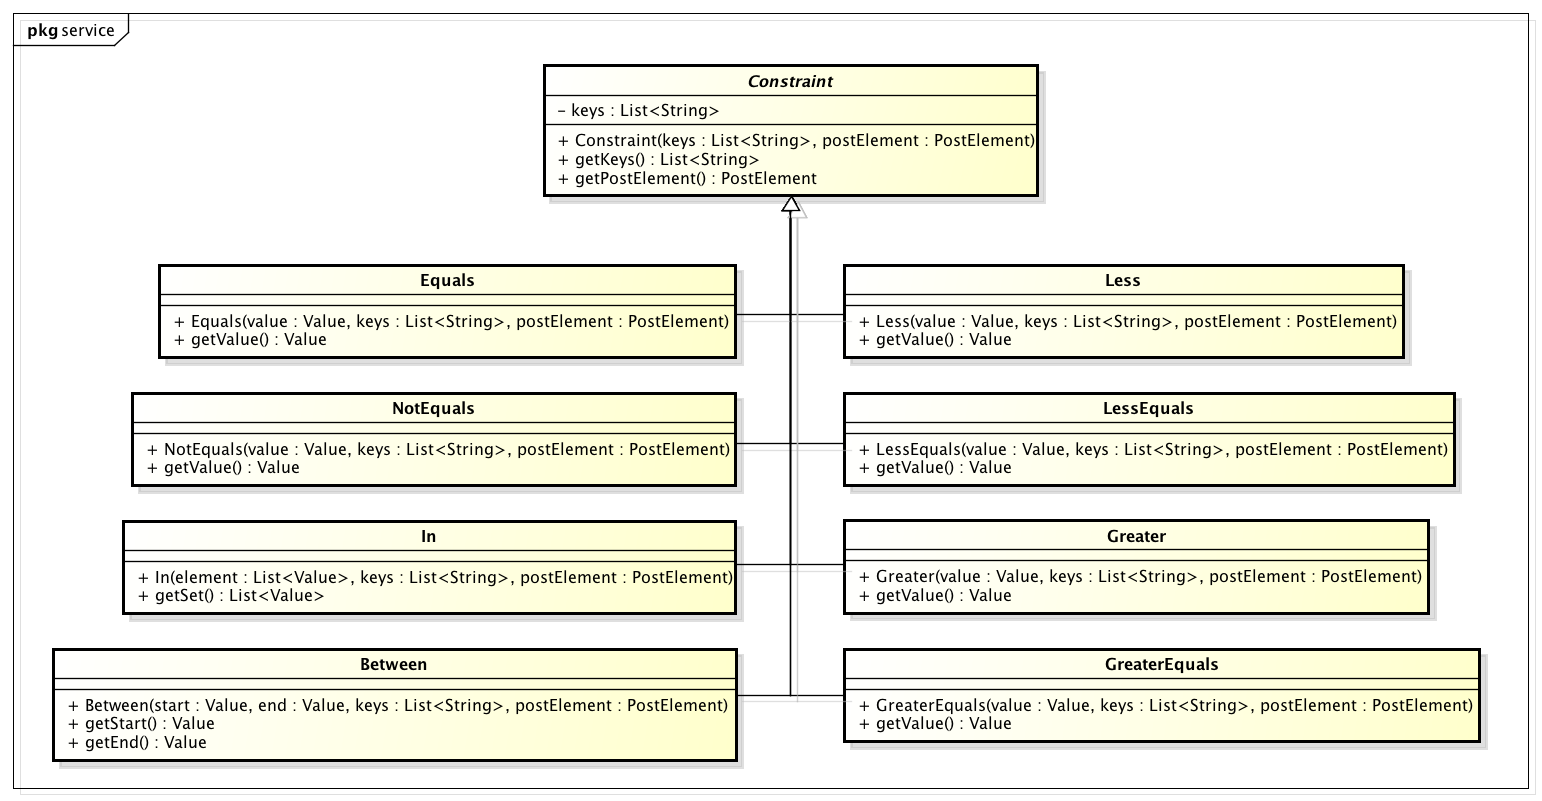
\includegraphics[width=1.0\textwidth]{figs/constraints}}
\caption{UML class diagram the allowed contraints in queries.}
\label{fig:constraints}
\end{figure}

The value searched must be a subtype of \emph{Value}. The constraints shown in \fig{fig:constraints} are applicable for all these subtypes. \emph{Greater}, \emph{GreaterEquals}, \emph{Less}, \emph{LessEquals} and \emph{Between} base on the alphabetical order for \emph{StringValue} type and the binary value for \emph{ByteArrayValue} type.

Multiple constraint can be combined with the \emph{and} operator. This is done by inserting multiple constraints in the list that is passed at creation of the \emph{Query} object.

The result returned by the \emph{Get} method is a \emph{ResultContainer} object. This object is formed of the list of posts returned by the database and an empty \emph{Attributes} object.
 

%%%%%%%%%%%%%%%%%%%%%%%%%%%%%%%%%%%%%%%%%%%%%%%%%%%%%%%%%%%%%%%%%%%%%%%%
\chapter{Distributed Bulletin Board}
%%%%%%%%%%%%%%%%%%%%%%%%%%%%%%%%%%%%%%%%%%%%%%%%%%%%%%%%%%%%%%%%%%%%%%%%

This chapters explains how a bulletin board is built as
a distributed system. The distributed system consists of
a set of nodes. Each node is assumed to be configured
accordingly.

The architectural model also assumes that a message to
be published is sent to one (trusted) node. (If the
application does not trust a given node then it can
choose among the other ones.) The message then is
processed by the Byzantine fault tolerant client
component \emph{BFTClient}. The BFT client component in turn
may use downstream components, and it will have
to use peers, the so called Byzantine fault tolerant
replica components of sort \emph{BFTReplica}.


\section{BFT Client Component}

In its first view, a \emph{BFTClient} acts as a component.
That is, it subclasses the generic component class
\emph{Component}. As such, it may use the service of
the successor (local) component. However, it will also
initiate an agreement protocol with peer replica
components of sort \emph{BFTReplica}. \fig{fig:byzantine-client}
shows the static structure of the Byzantine fault tolerant client
component.

\begin{figure}[ht]
\centerline{
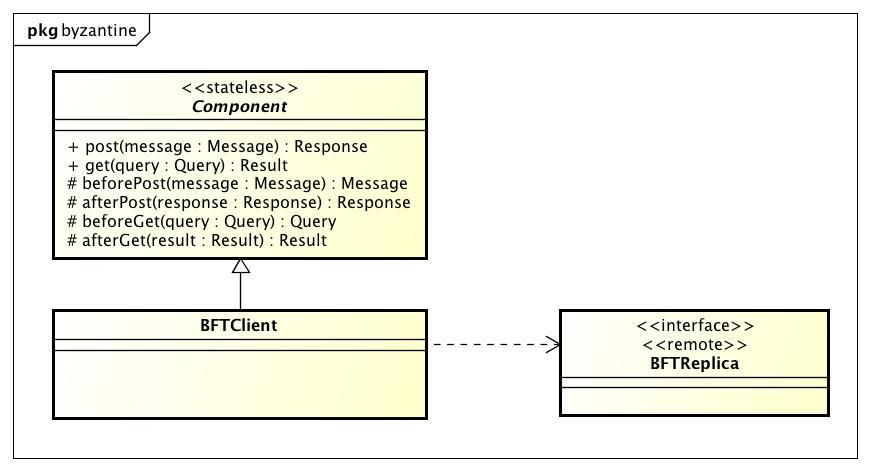
\includegraphics[width=1.0\textwidth]{figs/byzantine-client}}
\caption{UML class diagram illustrating the client side
of the replication component. Class \emph{BFTClient} extends the
\emph{Component} class. In addition, it uses the remote service
accessible via the \emph{BFTReplica} interface.}
\label{fig:byzantine-client}
\end{figure}


\section{BFT Replica Component}

Primarily, a Byzantine fault tolerant replica
component of sort \emph{BFTReplica} extends the
generic \emph{Component} implementation. In addition,
it also implements the \emph{BFTReplica} interface.
\fig{fig:byzantine-replica} shows
the static structure of the Byzantine fault tolerant replica
component.


\begin{figure}[ht<]
\centerline{
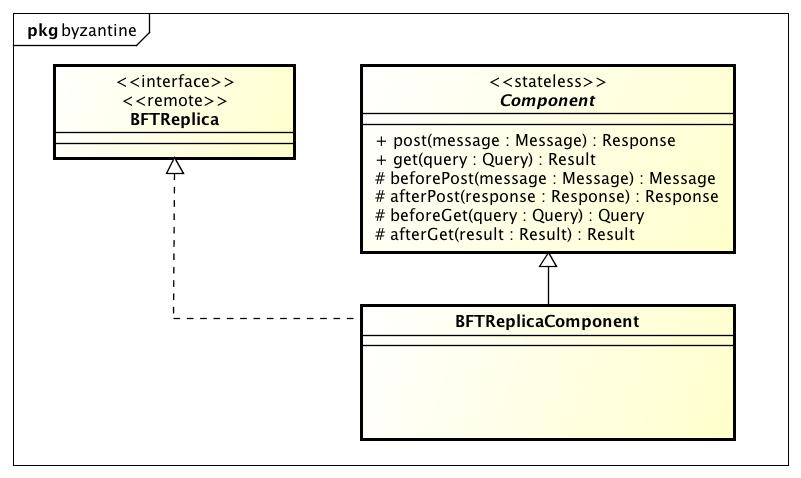
\includegraphics[width=1.0\textwidth]{figs/byzantine-replica}}
\caption{UML class diagram illustrating the replication side
of the replica component. Class \emph{BFTReplicaComponent}
extends the \emph{Component} class (and, thus, is a \emph{Service}). In
addition, it implements the \emph{BFTReplica} interface providing
specific services to peer replica clients.}
\label{fig:byzantine-replica}
\end{figure}

The communication between the BFT client and the BFT replicas
is an implementation detail and, therefore, not discussed here.
(It may involve yet another layered architecture and specialized
protocols, and it will use whatever communication technology
is appropriate.)


\section{Deployment View of the Replicated Board}

For the replicated configuration, each node is identically
configured with a set of required \emph{Component} instances, and
with the BFT client and BFT replica component instances.


%%%%%%%%%%%%%%%%%%%%%%%%%%%%%%%%%%%%%%%%%%%%%%%%%%%%%%%%%%%%%%%%%%%%%%%%
\chapter{Implementation Hints}
%%%%%%%%%%%%%%%%%%%%%%%%%%%%%%%%%%%%%%%%%%%%%%%%%%%%%%%%%%%%%%%%%%%%%%%%

Some implementation hints are given here.

\section{Namespaces, Names}

\begin{quote}
	\emph{Note.} The namespace \emph{org.uniboard} is already
	used in the domain name system of the Internet. Thus,
	we will have to discuss its use here.
\end{quote}

In order to ease the setup of the code base (project structure,
Maven artifacts, names to be defined), certain namespaces must be fixed.
The following namespace for the core service abstraction shall
be used:

\begin{lstlisting}
package org.uniboard.core;

public interface Service ...
public abstract class Component ...
public abstract class Request ...
public abstract class Response ...
public abstract class Query ...
public abstract class Result ...
\end{lstlisting}

Implementations will use additional namespaces such as
\emph{lu.unilu.uniboard.component1},
\emph{lu.unilu.uniboard.application1},
\emph{ch.bfh.uniboard.application2}, or
\emph{ch.bfh.uniboard.component2}.

Class names can also be concretized by following respective
technology conventions. When using EJB, the convention for
session bean classes is to use the suffix \emph{Bean}.


\section{Access to the Downstream Component}

In order to achieve upper-most flexibility, is is mandatory to
access the next downstream component by using the \emph{generic}
service interface. For example:

\begin{lstlisting}
package org.uniboard.core;

import javax.ejb.EJB;
import javax.ejb.LocalBean;
import javax.ejb.Stateless;

@Stateless
@LocalBean
public abstract class ComponentBean implements Service {

    @EJB
    private Service successor; // injected by the EJB container

    public Response post(Message message) ... {
        Message beforePost = beforePost(message);
        Response response = successor.post(beforePost);
        Response afterPost = afterPost(response);
        return afterPost;
    }
    ...
    protected Message beforePost(Message message) ... {
        return message;
    }
    protected Response afterPost(Response response) ... {
        return result;
    }
 }
\end{lstlisting}

Notice: By giving the component class the name \emph{ComponentBean}
we follow the propose name convention of EJB (TODO: Ref.\ to be
provided).

The injection performed by the container can be configured at
deploy-time. If EAR deployment units are used then the original
deployment descriptors or annotations can be overridden upon
configuring the EAR deployment unit.


\section{Skeleton for a Concrete Component}

The skeleton of a concrete component looks like:

\begin{lstlisting}
package ch.bfh.uniboard.authorization;

import org.uniboard.core.Service;
import org.uniboard.core.ComponentBean;

@Stateless
@LocalBean
public class AuthorizationServiceBean extends ComponentBean {
    // overwrite beforePost(), afterPost() accordingly
    // overwrite beforeGet(), afterGet() accordingly
}
\end{lstlisting}

Another example:

\begin{lstlisting}
package lu.unilu.uniboard.byzantine;

import org.uniboard.core.Service;
import org.uniboard.core.ComponentBean;

@Stateless
@LocalBean
public class BFTClientBean extends ComponentBean {
    // overwrite beforePost(), afterPost() accordingly
    // overwrite beforeGet(), afterGet() accordingly
}
\end{lstlisting}


\section{A Simple Scheme for Data Containers}

Application and components use the generic data containers
as described above (TODO Ref.\ to be provided) for the
communication of information to components. This is to keep a high
degree of flexibility and to reduce the coupling between
components.

The following flexible scheme for the implementation of generic
data containers shall be used:

\begin{lstlisting}
package org.uniboard.core;

import java.util.*;
import java.io.Serializable;

public class Message implements Serializable {
    private Map<String, Object> entries = new HashMap<>();
    public void put(String key, Object value) {...}
    public Object get(String key) {...}
}
\end{lstlisting}

Keys are strings to be agreed among components and application
programmers. (TODO: Envision a pre-defined set of keys.)
The types of the values are also
agreed among components and application programmers.
In order to reduce the
coupling, basic types and Java system types should be used.

Here is a sketch of code illustrating how components access
the information in, for example, a \emph{Message} container:

\begin{lstlisting}
    // in a component class
    @Override
    protected Message beforePost(Message message) ... {
        String id = (String) message.get("IDENTITY");
        byte[] signatureHashValue = (byte[]) message.get("SIGHASH");
        ...
        // Create new message, fill new message m accordingly...
        // Alternatively, the given message object may be updated...
        Message m = new Message();
        // Add information... Then:
        return m;
    }
\end{lstlisting}

The above sketch shows how keys (here \emph{IDENTITY} or \emph{SIGHASH})
can be used, and that applications or components must agree on
the types of values (here \emph{String} or \emph{byte[]}).

%%%%%%%%%%%%%%%%%%%%%%%%%%%%%%%%%%%%%%%%%%%%%%%%%%%%%%%%%%%%%%%%%%%%%%%%
\bibliographystyle{plain} \bibliography{arch-spec}
%%%%%%%%%%%%%%%%%%%%%%%%%%%%%%%%%%%%%%%%%%%%%%%%%%%%%%%%%%%%%%%%%%%%%%%%

\end{document}
